\documentclass[12pt,a4paper]{article}
\usepackage[utf8]{inputenc}
\usepackage[T1]{fontenc}
\usepackage{amsmath}
\usepackage{amsfonts}
\usepackage[francais]{babel}
\usepackage{amssymb}
\usepackage{graphicx}
\usepackage[top=2.00cm]{geometry}
\usepackage{enumitem}
%\usepackage{tikz}
\usepackage{mathtools}
%\usepackage{pgfplots}
%\usetikzlibrary{plotmarks}
\usepackage{bigcenter}
\usepackage{multicol}
\usepackage{minibox}

%Modif des enumerates numeros en gras. leftmargin=*,
\setlist[enumerate]{label=\textbf{\arabic*}.}

\usepackage{titlesec}
%modif des titres de section diminuer la taille
\titleformat{\section}
  {\normalfont\fontsize{14}{15}\bfseries}{\thesection}{1em}{}
\titleformat{\subsection}
  {\normalfont\fontsize{12}{15}\bfseries}{\thesubsection}{1em}{}


\author{CHARNAY Valentin, FINOT Sylvain}
\title{Compte rendu de TP : \\ Chaleur latente}

\begin{document}

\maketitle
L'objectif de ce TP est de mettre en évidence l'existence de la chaleur latente L(T) et de la quantifier dans le cas de l'eau.\\
Remarque : Toutes les incertitudes seront calculées avec la formule suivante : \\
$$\boxed{\Delta f \equiv \sqrt {\sum _{i}^{N}\left( \dfrac {\partial f} {\partial x_{i}}\right) ^{2}\cdot (\Delta x_i)^{2}}}$$
\section{Partie théorique}
\begin{enumerate}
\item Dans un premier temps, montrons que l'enthalpie libre (ou enthalpie de Gibbs) se conserve lors du changement d'état d'un fluide (corps pur). Cela revient à montrer qu'elle est constante le long d'un palier de liquéfaction. On a la relation :
\begin{align}
G = U + PV - TS
\end{align}
Donc, si on en prend la différentielle, on obtient : 
\begin{align*}
dG &= dU + d(PV) - d(TS)\\
&=dU + VdP + PdV - TdS - SdT 
\end{align*}
De plus $dU = TdS - PdV \implies dG=VdP-SdT$, donc à pression et température constant, $dP=dT=0 \implies dG=0$

\item En passant d'un palier de liquéfaction (isotherme T) à un autre infiniment proche ( isotherme T + dT), l'enthalpie libre va varier de dG. Ceci reste vrai que l'on se situe sur la courbe de rosée ou sur la courbe d'ébullition (extrémités d'un palier de liquéfaction). Ainsi, on peut écrire : $dG_L = dG_G$.
 D'où : 
\begin{align*}
V_LdP - S_LdT &= V_GdP - S_GdT\\
\Leftrightarrow \left( V_L - V_G \right)dP &= \left(S_L - S_G \right)dT\\
\Leftrightarrow \boxed{\frac{dP}{dT} = \frac{S_L - S_G}{V_L - V_G}}
\end{align*} 
\item D'après la relation $G = U + PV - TS$ on trouve :\\
\begin{align*}
G &= U + PV - TS\\
\Leftrightarrow G &= H - TS \\
\Rightarrow dG &= dH -TdS - SdT\\
\end{align*}
d'où à température et pression constante on trouve :
$$ dG = dH - TdS = 0 $$
$$ \Rightarrow dS = \frac{dH}{T} \Leftrightarrow \int dS = \int \frac{dH}{T}$$
$$\boxed{ \Delta S = \frac{\Delta H}{T} = \frac{L}{T}}$$
Où L est la chaleur latente aussi appelée enthalpie de changement d'état. On trouve donc : \\
\begin{align}
L&=T.\dfrac{dP}{dT}(V_g - V_l)
\end{align}
\end{enumerate}

\section{Partie expérimentale}
\begin{itemize}
\item Le principe de l'expérience est de chauffer un volume d'eau dans un ballon et une fois le vide d'air effectué (obtenu à $\approx$ 100 $ ^\circ C$), mesurer les valeurs de pression et de température décroissantes dans le temps.\\
\begin{bigcenter}
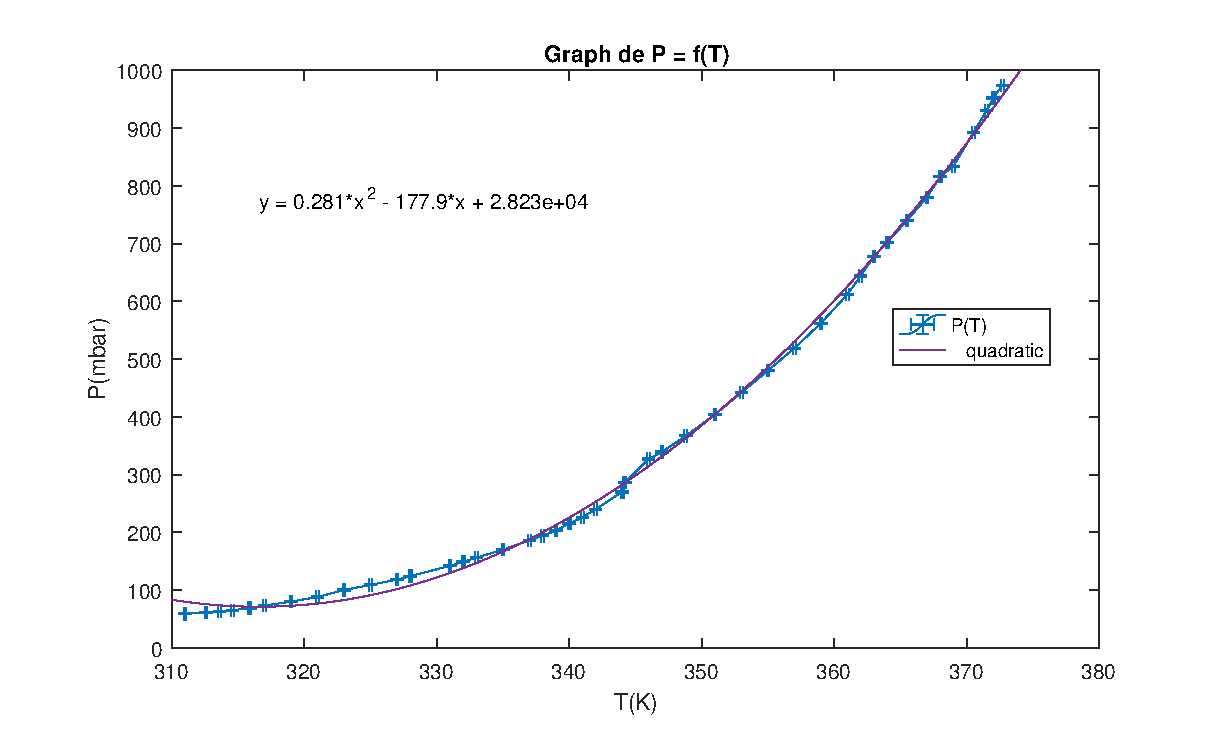
\includegraphics[scale=0.8]{PfT}
\end{bigcenter}
Nous nous intéressons maintenant à la  façon de trouver la chaleur latente de l'eau à partir de nos mesures. \\
Remarque : Dans un premier temps, nous voulions déterminer $\dfrac{dP}{dT}$ en rapprochant nos mesures d'un modèle.\\ Un modèle quadratique se rapproche nettement de nos valeurs, cependant, l'écart est plus important aux basses températures. En réalité après quelques recherches, il s'agit davantage d'une exponentielle. Cependant cela n'a pas réellement d'importance puisque nous n'utiliserons pas cette méthode.

\begin{align*}
L&=T.\dfrac{dP}{dT}(V_g - V_l)\\ \\
%
L_{mol}&=T.\dfrac{dP}{dT}(v_g - v_l)=T.\dfrac{dP}{dT}.v_g(1 - \dfrac{v_l}{v_g})\\ \\
%
&\approx T.\dfrac{dP}{dT}.v_g \qquad \text{car } \dfrac{v_l}{v_g} \approx 10^{-3} << 1\\ \\
%
L_{mol}&=T.\dfrac{dP}{dT}.\dfrac{RT}{P} \qquad \text{approximation Gaz Parfait}\\
\end{align*}
$$\implies \dfrac {dP} {P}=\dfrac {L_{mol}} {R}\dfrac {dT} {T^{2}} \iff \int\dfrac {dP} {P}=\int\dfrac {L_{mol}} {R}\dfrac {dT} {T^{2}}  $$\\
$$\boxed{\ln(P)=-\dfrac{L_{mol}}{RT}+C}$$\\
En traçant $\ln(P)=f(1/T) $ on s'attend donc à trouver une droite de pente $-\dfrac{L_{mol}}{R}$.\\
Par la suite on pourra également tracer $L_{mol}=(C-\ln(P)).RT$
\begin{bigcenter}
\includegraphics[scale=0.8]{lnp}
\end{bigcenter}
%\pagebreak
Calculs des barres d'erreurs (en utilisant la formule vu en introduction) :\\
$$\Delta(1/T)=\sqrt{\dfrac{\Delta T^2}{T^4}}\qquad \Delta(\ln(P))=\dfrac {\Delta P} {P}$$
Les paramètres de la régression sont les suivants :\\
\minibox[frame]{
Linear model Poly1:\\
     f(x) = p1*x + p2\\
Coefficients (with 95\% confidence bounds):\\
       p1 =       -5525$\pm95,5$  (-5621, -5430)\\
       p2 =       26.31$\pm0,28$  (26.03, 26.59)\\
       }\linebreak
\vspace{2mm}

On peut donc déjà calculer la chaleur latente (ici supposée constante) : \\
\begin{align*}
-\dfrac{L_{mol}}{R}&=-5525\pm95,5\\
 \iff L_{M}&=\dfrac{5528\times8,314}{18}=2552\pm0,04 \text{ kJ/kg}
\end{align*} 
On peut la comparer à une valeur tabulée : 2454,3 kJ/kg à 20$ ^\circ C$ (Wikipédia)\\
On obtient bien le même ordre de grandeur.\\
Traçons à présent : $$L_{M}=(p2-\ln(P))\dfrac{R.T}{18} \quad \text{et} \quad
\Delta L = \dfrac{R}{18} \sqrt{\dfrac{T^2 \Delta P^2}{P^2}+\Delta T^2 (p_2-\ln (P))^2+T^2 \Delta p_2^2}$$
Exemple à T = 355K, P=480mbar : 
\begin{align*}
L_{M}&=(p2-\ln(P))\dfrac{R.T}{18}\\
&=(26,31-10,78)\dfrac{8,314\times355}{18}=2547 \text{kJ/kg}\\ 
\\
\Delta L &=\dfrac{R}{18} \sqrt{\dfrac{T^2 \Delta P^2}{P^2}+\Delta T^2 (p_2-\ln (P))^2+T^2 \Delta p_2^2}\\
&=\dfrac{8,314}{18} \sqrt{\dfrac{355^2.(10^2)^2}{(4,8.10^4)^2}+0,1^2 . (26,31-\ln (4,8.10^4))^2+355^2.0,28^2}\\
&=45,9 \text{kJ/kg}
\end{align*}
$$\implies \boxed{L_M = 2547\pm45,9\text{kJ/kg}}$$\\
Le graph ci-dessous est obtenu en appliquant la même méthode en chaque point. 
\begin{bigcenter}
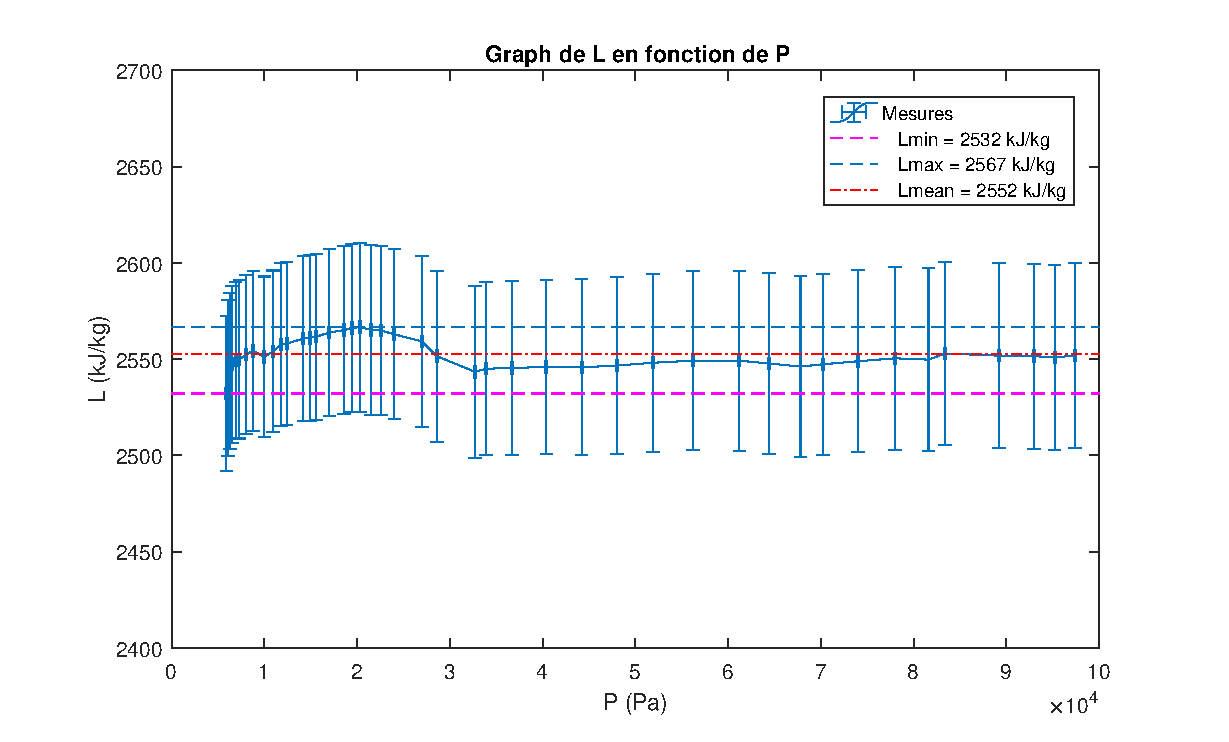
\includegraphics[scale=0.7]{L}
\end{bigcenter}
\end{itemize}
Comparons nos résultats avec une table :
\begin{bigcenter}
\begin{table}[]
\centering
\begin{tabular}{ccc}
\textbf{Absolute Pressure} & \textbf{Boiling Point} & \textbf{Latent heat of Vaporization} \\
\textbf{(bar)}             & \textbf{($^\circ$C)}          & \textbf{(kJ/kg)}                     \\
%0.02                       & 17.51                  & 2460.19                              \\
%0.03                       & 24.10                  & 2444.65                              \\
%0.04                       & 28.98                  & 2433.10                              \\
0.05                       & 32.90                  & 2423.82                              \\
0.06                       & 36.18                  & 2416.01                              \\
0.07                       & 39.02                  & 2409.24                              \\
0.08                       & 41.53                  & 2403.25                              \\
0.09                       & 43.79                  & 2397.85                              \\
0.1                        & 45.83                  & 2392.94                              \\
0.2                        & 60.09                  & 2358.40                              \\
0.3                        & 69.13                  & 2336.13                              \\
0.4                        & 75.89                  & 2319.23                              \\
0.5                        & 81.35                  & 2305.42                              \\
0.6                        & 85.95                  & 2293.64                              \\
0.7                        & 89.96                  & 2283.30                              \\
0.8                        & 93.51                  & 2274.05                              \\
0.9                        & 96.71                  & 2265.65                              \\
1                          & 99.63                  & 2257.92                             
\end{tabular}
\caption{Chaleur latente de vaporisation en fonction de la pression}
Source : engineeringtoolbox
\label{my-label}
\end{table}
\end{bigcenter}
On remarque que toutes nos valeurs sont décalées au dessus des valeurs données. Cela peut être du au fait que nous avons supposé la vapeur d'eau comme un gaz parfait pour estimer son volume molaire. En négligeant également le volume de liquide devant le volume de gaz, on introduit une erreur de l'ordre de $10^{-3}$.\\
Autre remarque, nos incertitudes ne nous permettent pas de voir le caractère décroissant de la chaleur latente en fonction de l'augmentation de pression.
En conclusion, en tenant compte de nos incertitudes et de nos hypothèses simplificatrices, on arrive tout de même à obtenir une bonne approximation de la chaleur latente.\\
En comparant le point calculé à la main avec le point le plus proche dans la table (0,5bar, 81,35$^\circ C$ (354,35K)) : 
$$\dfrac{2547\pm45,9-2305}{2305}\times100=10,5\pm2 \% $$
Une erreur de l'ordre de 10\%, compte tenu de nos incertitudes nous semble plutôt raisonnable.
\section{Expérience de vulgarisation}
\begin{itemize}
\item

Afin de vulgariser le principe de chaleur latente, nous proposons l'expérience suivante :\\
\begin{multicols}{2}
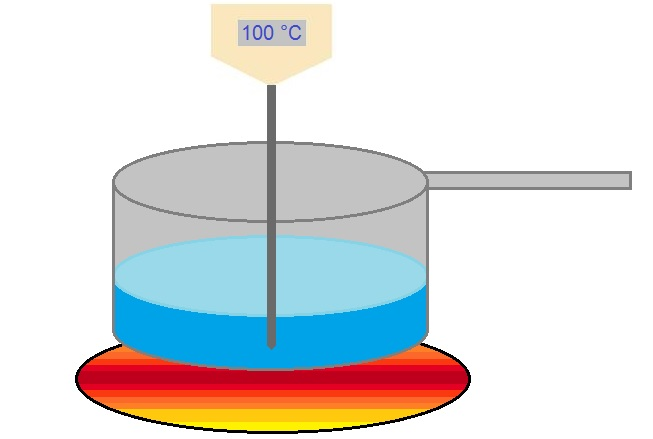
\includegraphics[scale=0.5]{exp2} 
\columnbreak

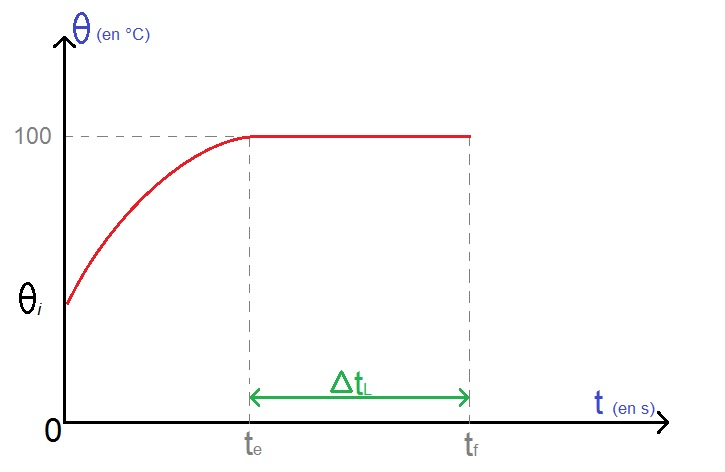
\includegraphics[scale=0.5]{graph1}
 \end{multicols}
 
On place un petit volume d'eau dans une casserole que l'on chauffe. On relève la température de l'eau liquide à intervalle de temps régulier afin de tracer la courbe $ \theta $ en fonction de t. On devrait obtenir une courbe de ce genre (ci-dessus) où la chaleur latente L est caractérisé par le palier constant à 100 $ ^\circ C$ jusqu'à l'évaporation total de l'eau.\\
 
 Cette expérience montre bien la nécessité d'apporter plus d'énergie à un système pour lui permettre de changer d'état, énergie que l'on appelle chaleur latente.
 
 \item
 Pour quantifier cette énergie, il suffit de mesurer la puissance électrique fourni à la plaque électrique à l'aide d'un [...]. En supposant qu'il n'y a pas de pertes de puissance en passant par la plaque puis par la casserole. Ensuite nous n'avons plus qu'a calculer l'énergie $E_W = W_{elec}.\Delta t_L$  où $\Delta t_L$ correspond à l'intervalle temps  où la température de l'eau est constante.\\
 
 \item
 En faisant l'expérience, on obtient le graph suivant \\
 \\
 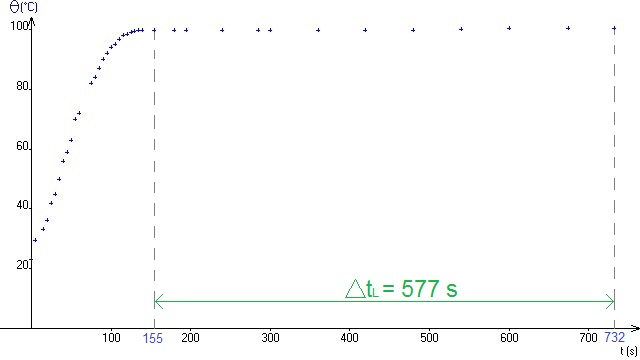
\includegraphics[scale=0.7]{graph2}\\
 
 \item
 En ayant relevé une puissance électrique de 1 042 Watts, on obtient l'application numérique suivante :
 $$ AN : E_W \approx 1042 * 577 \approx 601 234 J \approx 601 kJ$$
 La chaleur latente étant de 2550 kJ/kg (dans les tables de données) et ayant approximativement un volume de 200 mL d'eau distillé (soit 200 g); nous devons trouver une énergie transmise au système de 2 550 * 0.200 $\approx$ 510 kJ.\\
 
 Notre expériences ne permettait d'obtenir qu'un ordre de grandeur de $L_{eb}$ sachant toutes les approximation faites ($m_{H_2O},W_{elec}=W_{transmis}$) on retrouve bien une valeur de $L_{eb}$ proche de la théorie.  
 
 

 \end{itemize}
\end{document}